\chapter{Chaos analysis of multiple coupled blocks}
\label{chap: multi block}

\section{Two blocks}

\begin{figure}[H]
    \centering
    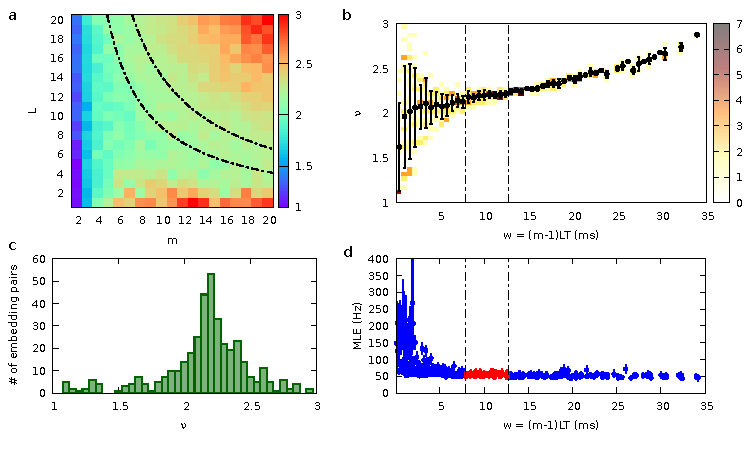
\includegraphics[width=\linewidth]{../2_blocks/1e5_points/plots/chaos.pdf}
    \caption{Edge}
    \label{fig:2 blocks chaos}
\end{figure}


\section{Three blocks}

\begin{figure}[H]
    \centering
    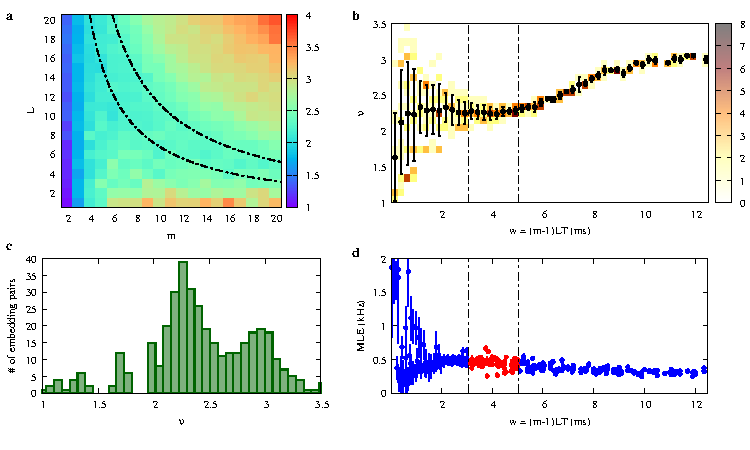
\includegraphics[width=\linewidth]{../3_blocks/edge/2e5_points/plots/chaos_low.pdf}
    \caption{Edge}
    \label{fig:3 blocks chaos}
\end{figure}

\begin{figure}[H]
    \centering
    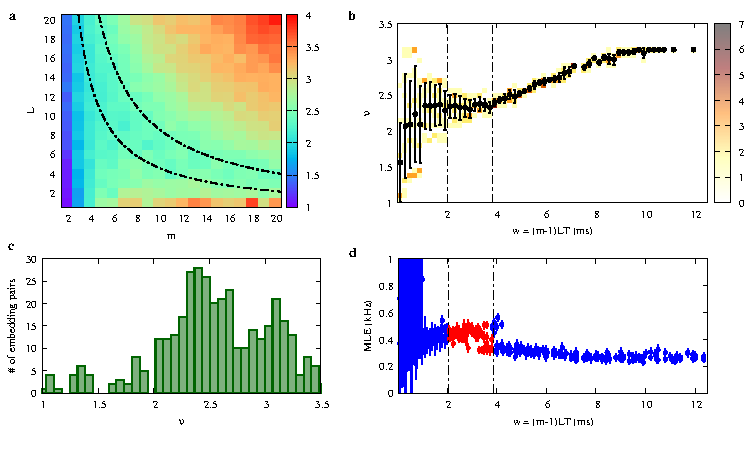
\includegraphics[width=\linewidth]{../3_blocks/middle/2e5_points/plots/chaos_low.pdf}
    \caption{Middle}
    \label{fig:3 blocks chaos middle}
\end{figure}

\section{Four blocks}

\begin{figure}[H]
    \centering
    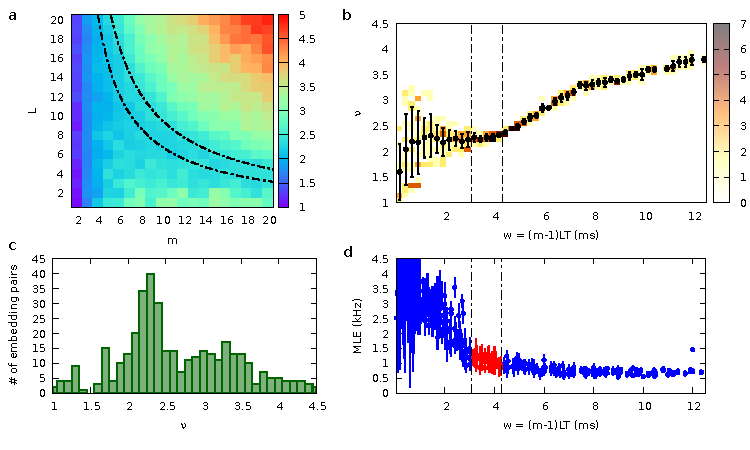
\includegraphics[width=\linewidth]{../4_blocks/2e5_points_new/plots/chaos_low.pdf}
    \caption{Edge}
    \label{fig:4 blocks chaos}
\end{figure}


\section{Five blocks}

\begin{figure}[H]
    \centering
    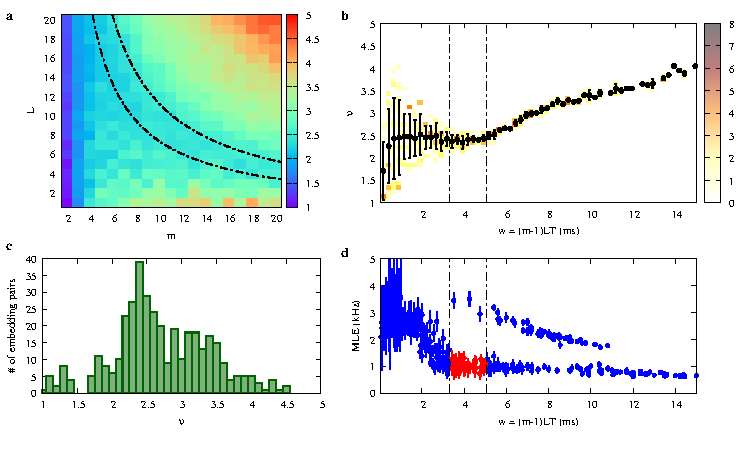
\includegraphics[width=\linewidth]{../5_blocks/edge/2e5_points/plots/chaos_low.pdf}
    \caption{Edge}
    \label{fig:5 blocks chaos}
\end{figure}

\begin{figure}[H]
    \centering
    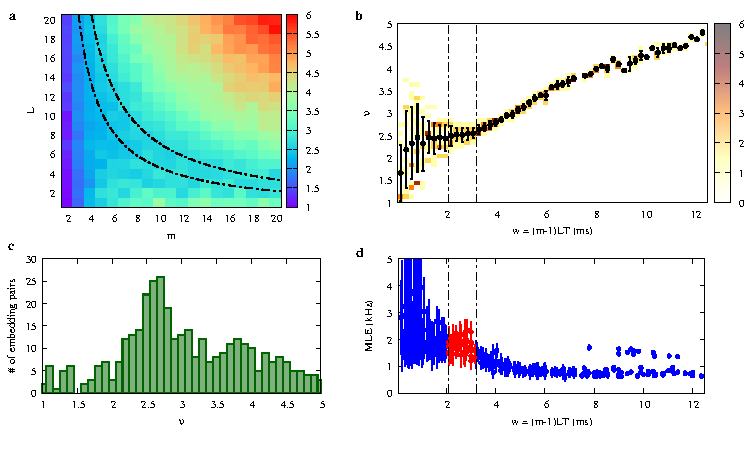
\includegraphics[width=\linewidth]{../5_blocks/middle/2e5_points/plots/chaos_low.pdf}
    \caption{Middle}
    \label{fig:5 blocks chaos middle}
\end{figure}

\section{Six blocks}

\begin{figure}[H]
    \centering
    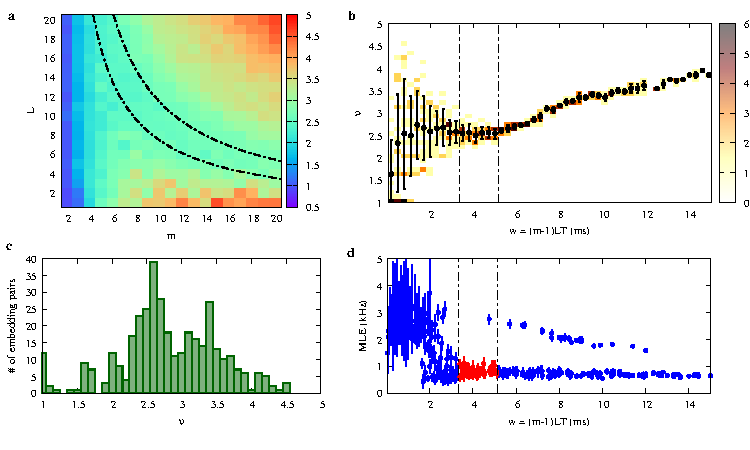
\includegraphics[width=\linewidth]{../6_blocks/2e5_points/plots/chaos_low.pdf}
    \caption{Edge}
    \label{fig:6 blocks chaos}
\end{figure}

\section{Seven blocks}

\begin{figure}[H]
    \centering
    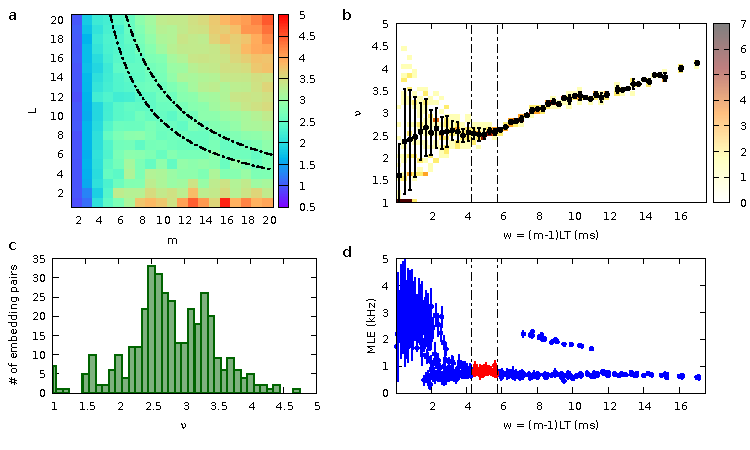
\includegraphics[width=\linewidth]{../7_blocks/edge/2e5_points/plots/chaos_low.pdf}
    \caption{Edge}
    \label{fig:7 blocks chaos}
\end{figure}

\begin{figure}[H]
    \centering
    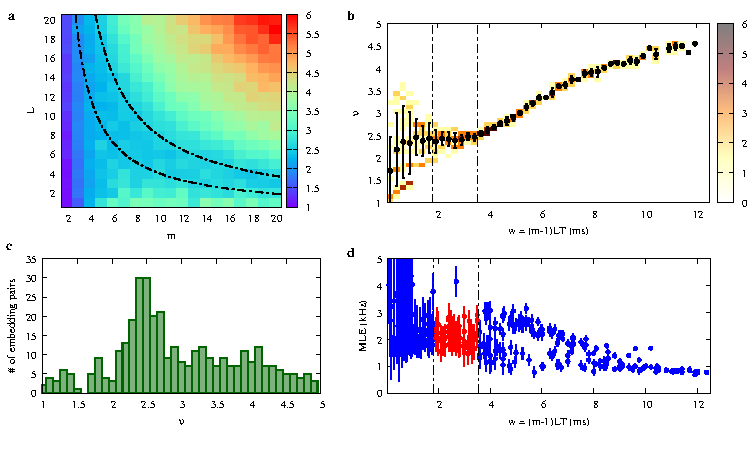
\includegraphics[width=\linewidth]{../7_blocks/middle/2e5_points/plots/chaos_low.pdf}
    \caption{Middle}
    \label{fig:7 blocks chaos middle}
\end{figure}

\section{Eight blocks}

\begin{figure}[H]
    \centering
    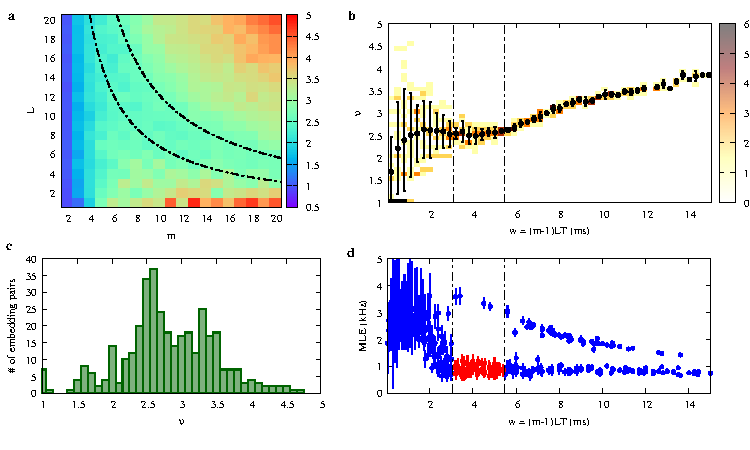
\includegraphics[width=\linewidth]{../8_blocks/2e5_points/plots/chaos_low.pdf}
    \caption{Edge}
    \label{fig:8 blocks chaos}
\end{figure}

\section{Nine blocks}

\begin{figure}[H]
    \centering
    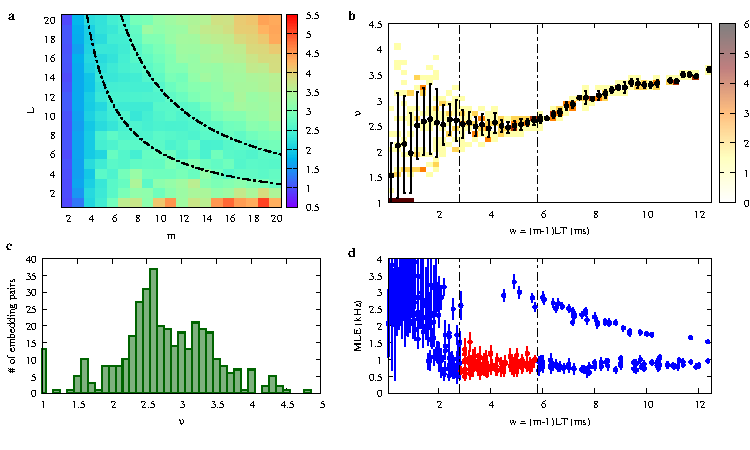
\includegraphics[width=\linewidth]{../9_blocks/edge/2e5_points/plots/chaos_low.pdf}
    \caption{Edge}
    \label{fig:9 blocks chaos}
\end{figure}

\begin{figure}[H]
    \centering
    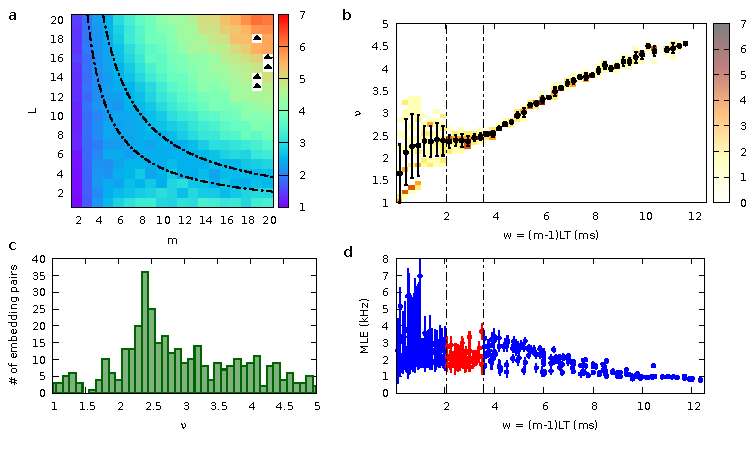
\includegraphics[width=\linewidth]{../9_blocks/middle/2e5_points/plots/chaos_low.pdf}
    \caption{Middle}
    \label{fig:9 blocks chaos middle}
\end{figure}

\section{Ten blocks}

\begin{figure}[H]
    \centering
    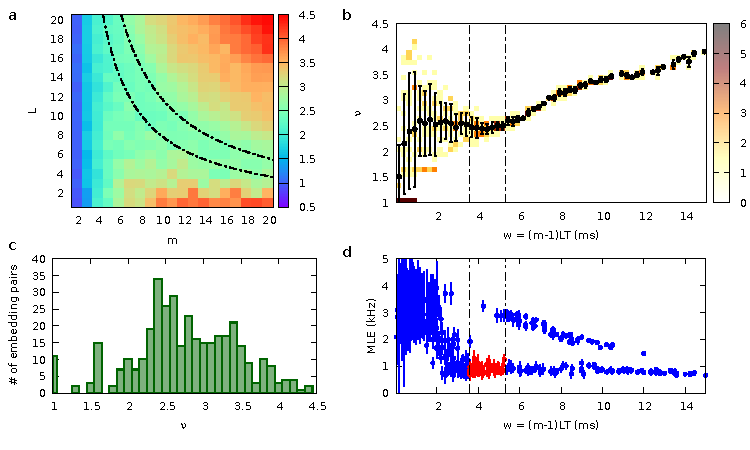
\includegraphics[width=\linewidth]{../10_blocks/2e5_points/plots/chaos_low.pdf}
    \caption{Edge}
    \label{fig:10 blocks chaos}
\end{figure}

\section{Eleven blocks}

\begin{figure}[H]
    \centering
    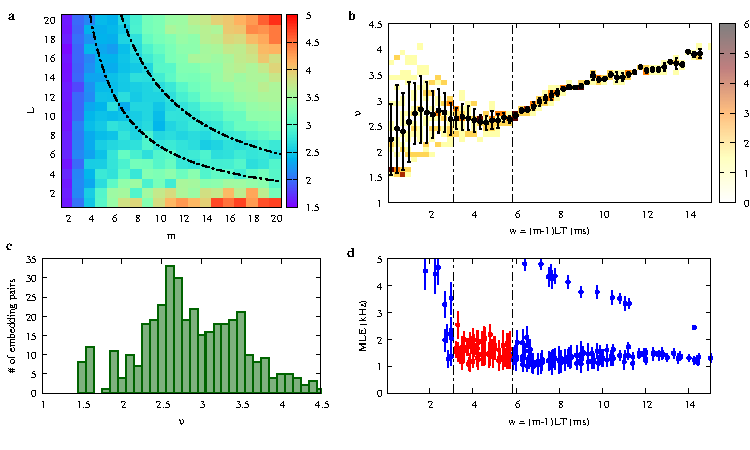
\includegraphics[width=\linewidth]{../11_blocks/edge/2e5_points/plots/chaos_low.pdf}
    \caption{Edge}
    \label{fig:11 blocks chaos}
\end{figure}

\begin{figure}[H]
    \centering
    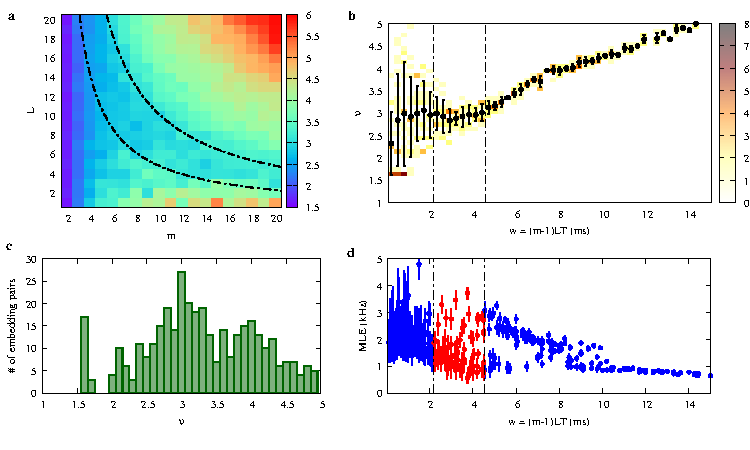
\includegraphics[width=\linewidth]{../11_blocks/middle/2e5_points/plots/chaos_low.pdf}
    \caption{Middle}
    \label{fig:11 blocks chaos middle}
\end{figure}

\section{Twelve blocks}

\begin{figure}[H]
    \centering
    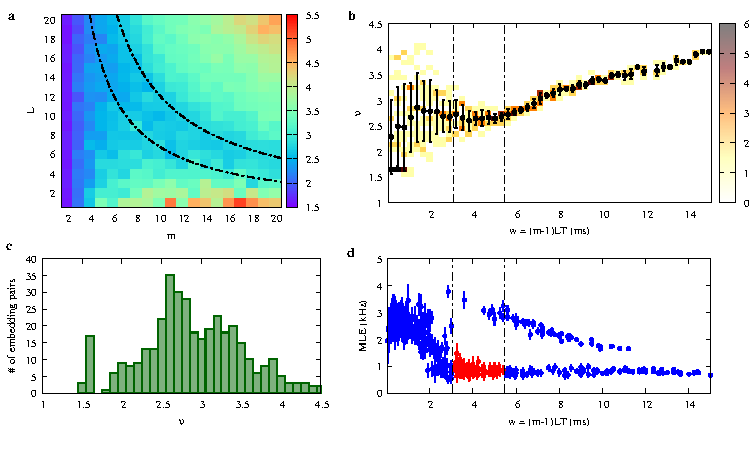
\includegraphics[width=\linewidth]{../12_blocks/2e5_points/plots/chaos_low.pdf}
    \caption{Edge}
    \label{fig:12 blocks chaos}
\end{figure}

\section{Thirteen blocks}

\begin{figure}[H]
    \centering
    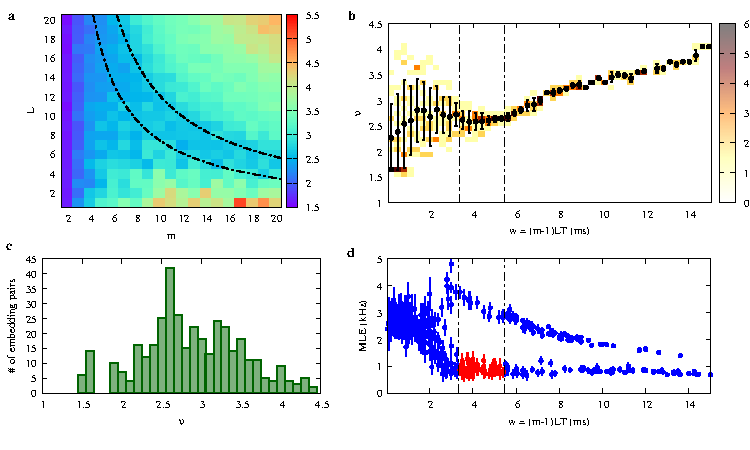
\includegraphics[width=\linewidth]{../13_blocks/edge/2e5_points/plots/chaos_low.pdf}
    \caption{Edge}
    \label{fig:13 blocks chaos}
\end{figure}


\section{Fifteen blocks}

\begin{figure}[H]
    \centering
    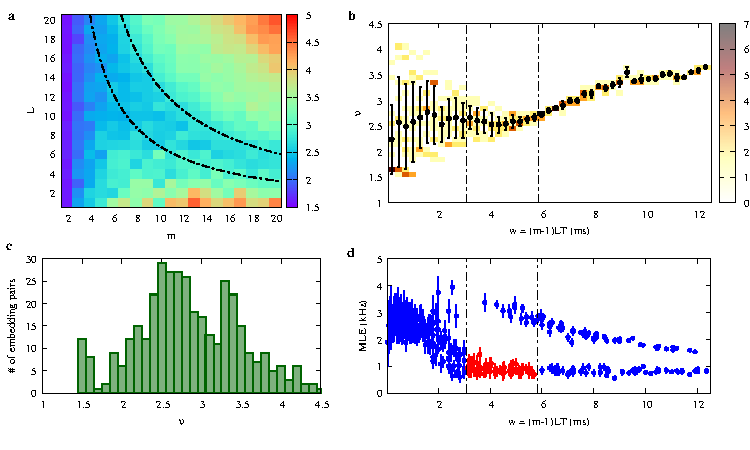
\includegraphics[width=\linewidth]{../15_blocks/edge/2e5_points/plots/chaos_low.pdf}
    \caption{Edge}
    \label{fig:15 blocks chaos}
\end{figure}

\begin{figure}[H]
    \centering
    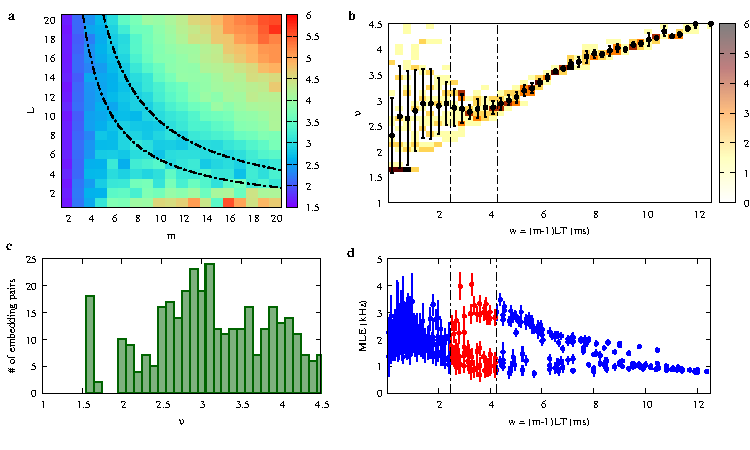
\includegraphics[width=\linewidth]{../15_blocks/middle/2e5_points/plots/chaos_low.pdf}
    \caption{Middle}
    \label{fig:15 blocks middle chaos}
\end{figure}

\section{Twenty blocks}

\begin{figure}[H]
    \centering
    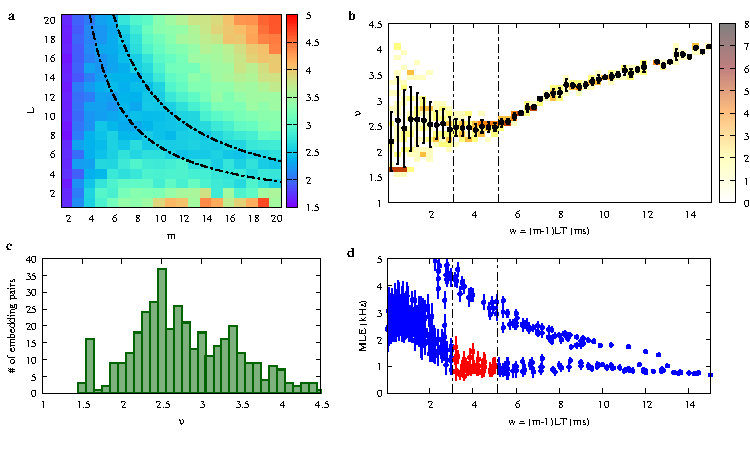
\includegraphics[width=\linewidth]{../20_blocks/2e5_points/plots/chaos_low.pdf}
    \caption{Edge}
    \label{fig:20 blocks chaos}
\end{figure}

\section{Twentyfive blocks}

\begin{figure}[H]
    \centering
    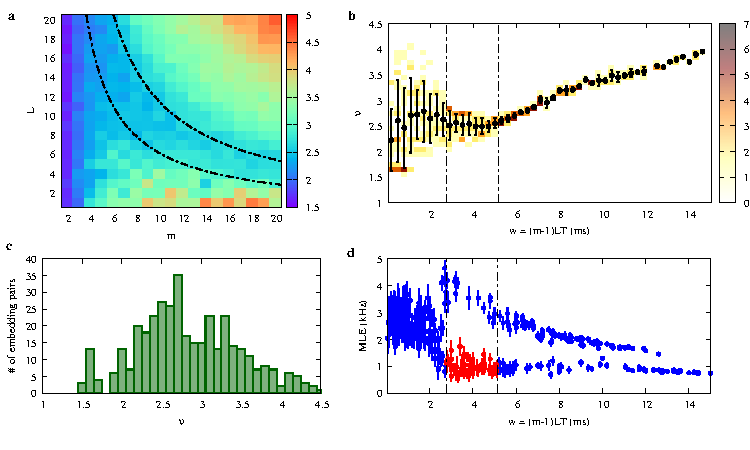
\includegraphics[width=\linewidth]{../25_blocks/edge/2e5_points/plots/chaos_low.pdf}
    \caption{Edge}
    \label{fig:25 blocks chaos}
\end{figure}

\begin{figure}[H]
    \centering
    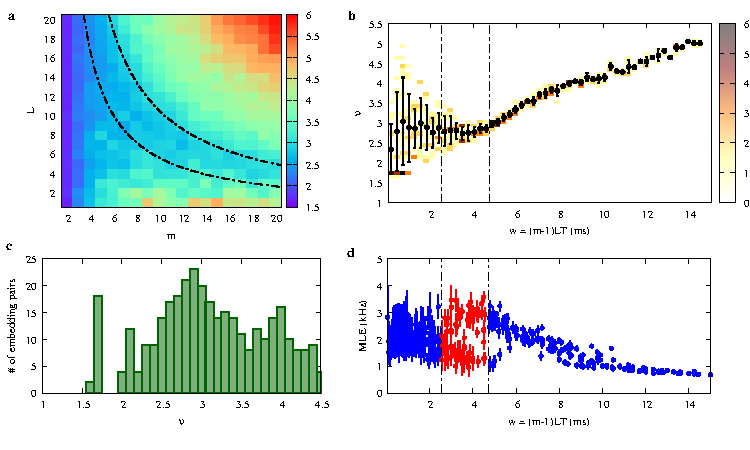
\includegraphics[width=\linewidth]{../25_blocks/middle/2e5_points/plots/chaos_low.pdf}
    \caption{Middle}
    \label{fig:25 blocks chaos middle}
\end{figure}


\section{Conclusions}

\begin{figure}[H]
    \centering
    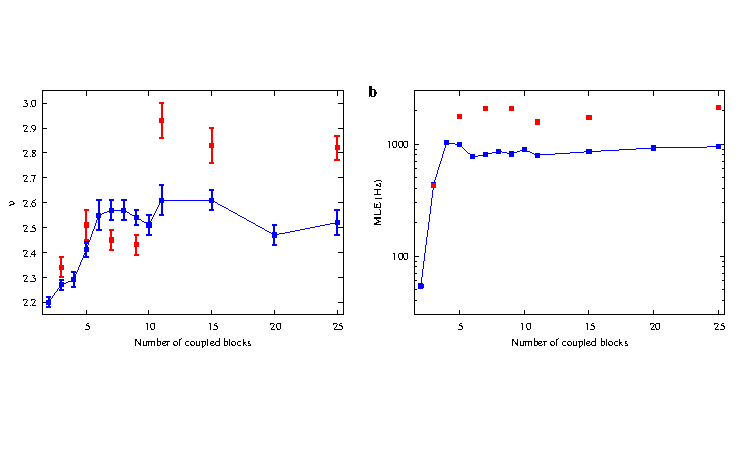
\includegraphics[width=\linewidth,trim={0 1.5cm 0 1.3cm},clip]
    {../data/nu_mle_blocks.pdf}
    \caption{Edge (blue) and middle (red)}
    \label{fig:nu mle blocks}
\end{figure}
